A function of the form $y=f(x)$ is a function of a single variable; given a value of $x$, we can find a value $y$. Even the vector--valued functions of Chapter \ref{chap:vvf} are single--variable functions; the input is a single variable though the output is a vector.

There are many situations where a desired quantity is a function of two or more variables. For instance, wind chill is measured by knowing the temperature and wind speed; the volume of a gas can be computed knowing the pressure and temperature of the gas; to compute a baseball player's batting average, one needs to know the number of hits and the number of at--bats. 

This chapter studies \textbf{multivariable} functions, that is, functions with more than one input.

\section{Introduction to Multivariable Functions}\label{sec:multi_intro}

\definition{def:multi2}{Function of Two Variables}
{Let $D$ be a subset of $\mathbb{R}^2$. A \textbf{function $f$ of two variables} is a rule that assigns each pair $(x,y)$ in $D$ a value $z=f(x,y)$ in $\mathbb{R}$. $D$ is the \textbf{domain} of $f$; the set of all outputs of $f$ is the \textbf{range}.
\index{multivariable function}\index{multivariable function!domain}\index{multivariable function!range}\index{function!of two variables}
}

\example{ex_multi1}{Understanding a function of two variables}{
Let $z=f(x,y) = x^2-y$. Evaluate $f(1,2)$, $f(2,1)$, and $f(-2,4)$; find the domain and range of $f$.}
{Using the definition $f(x,y) = x^2-y$, we have:
\begin{align*}
f(1,2) &= 1^2-2 = -1\\
f(2,1) &=	2^2-1 = 3\\
f(-2,4) &= (-2)^2-4 = 0
\end{align*}
The domain is not specified, so we take it to be all possible pairs in $\mathbb{R}^2$ for which $f$ is defined. In this example, $f$ is defined for \emph{all} pairs $(x,y)$, so the domain $D$ of $f$ is $\mathbb{R}^2$. 
\enlargethispage{3\baselineskip}

The output of $f$ can be made as large or small as possible; any real number $r$ can be the output. (In fact, given any real number $r$, $f(0,-r)=r$.) So the range $R$ of $f$ is $\mathbb{R}$.
}\\

\example{ex_multi2}{Understanding a function of two variables}{
Let $\ds f(x,y) = \sqrt{1-\frac{x^2}9-\frac{y^2}4}.$ Find the domain and range of $f$.}
{The domain is all pairs $(x,y)$ allowable as input in $f$. Because of the square--root, we need $(x,y)$ such that $0\leq1-\frac{x^2}9-\frac{y^2}4$:
\begin{align*}
0&\leq1-\frac{x^2}9-\frac{y^2}4\\
\frac{x^2}9+\frac{y^2}4 &\leq 1
\end{align*}
The above equation describes an ellipse and its interior as shown in Figure \ref{fig:multi2}. We can represent the domain $D$ graphically with the figure; in set notation, we can write $D = \{(x,y)|\,\frac{x^2}9+\frac{y^2}4 \leq 1\}$.
\mfigure{.75}{Illustrating the domain of $f(x,y)$ in Example \ref{ex_multi2}.}{fig:multi2}{figures/figmulti2}

The range is the set of all possible output values. The square--root ensures that all output is $\geq 0$. Since the $x$ and $y$ terms are squared, then subtracted, inside the square--root, the largest output value comes at $x=0$, $y=0$: $f(0,0) = 1$. Thus the range $R$ is the interval $[0,1]$.
}\\

\noindent\textbf{\large Graphing Functions of Two Variables}\\

The \textbf{graph} of a function $f$ of two variables is the set of all points $\big(x,y,f(x,y)\big)$ where $(x,y)$ is in the domain of $f$. This creates a \textbf{surface} in space.
\mtable{.4}{Graphing a function of two variables.}{fig:multigraph_intro}{%
\begin{tabular}{c}
\myincludegraphicsthree{width=150pt,3Dmenu,activate=onclick,deactivate=pageinvisible,
3Droll=0.5548354761871764,
3Dortho=0.004999999888241291,
3Dc2c=0.5822595357894897 0.666623592376709 0.4653888940811157,
3Dcoo=-4.197300910949707 1.0700405836105347 59.15589141845703,
3Droo=129.99999935798337,
3Dlights=Headlamp,add3Djscript=asylabels.js}{}{figures/figmultigraph_intro}\\
%\myincludegraphics[trim=1mm 0mm 1mm 3mm,clip,scale=1.25]{figures/figmultigraph_intro}\\
(a)\\[10pt]
\myincludegraphicsthree{width=150pt,3Dmenu,activate=onclick,deactivate=pageinvisible,
3Droll=0.5548354761871764,
3Dortho=0.004999999888241291,
3Dc2c=0.5822595357894897 0.666623592376709 0.4653888940811157,
3Dcoo=-4.197300910949707 1.0700405836105347 59.15589141845703,
3Droo=129.99999935798337,
3Dlights=Headlamp,add3Djscript=asylabels.js}{}{figures/figmultigraph_introb}\\
%\myincludegraphics[trim=1mm 0mm 1mm 3mm,clip,scale=1.25]{figures/figmultigraph_introb}\\
(b)
\end{tabular}
}

One can begin sketching a graph by plotting points, but this has limitations. Consider Figure \ref{fig:multigraph_intro}(a) where 25 points have been plotted of $\ds f(x,y) = \frac1{x^2+y^2+1}$. More points have been plotted than one would reasonably want to do by hand, yet it is not clear at all what the graph of the function looks like. Technology allows us to plot lots of points, connect adjacent points with lines and add shading to create a graph like Figure \ref{fig:multigraph_intro}b which does a far better job of illustrating the behavior of $f$.

While technology is readily available to help us graph functions of two variables, there is still a paper--and--pencil approach that is useful to understand and master as it, combined with high--quality graphics, gives one great insight into the behavior of a function. This technique is known as sketching \textbf{level curves}.\\

\noindent\textbf{\large Level Curves}\\

It may be surprising to find that the problem of representing a three dimensional surface on paper is familiar to most people (they just don't realize it).\index{multivariable function!level curves}\index{level curves}\index{contour lines} Topographical maps, like the one shown in Figure \ref{fig:topomap}, represent the surface of Earth by indicating points with the same elevation with \sword{contour lines}. The elevations marked are equally spaced; in this example, each thin line indicates an elevation change in 50ft increments and each thick line indicates a change of 200ft. When lines are drawn close together, elevation changes rapidly (as one does not have to travel far to rise 50ft). When lines are far apart, such as near ``Aspen Campground,'' elevation changes more gradually as one has to walk farther to rise 50ft.

\mfigure[scale=.65]{.75}{A topographical map displays elevation by drawing contour lines, along with the elevation is constant.\\ \tiny Sample taken from the public domain USGS Digital Raster Graphics, \texttt{http://topmaps.usgs.gove/drg/}.}{fig:topomap}{figures/MT_ChromeMountain_topo_smallx}
%\mtable{.75}{A topographical map displays elevation by drawing contour lines, along with the elevation is constant.\\ \tiny Sample taken from the public domain USGS Digital Raster Graphics, \texttt{http://topmaps.usgs.gove/drg/}.}{fig:topomap}{
%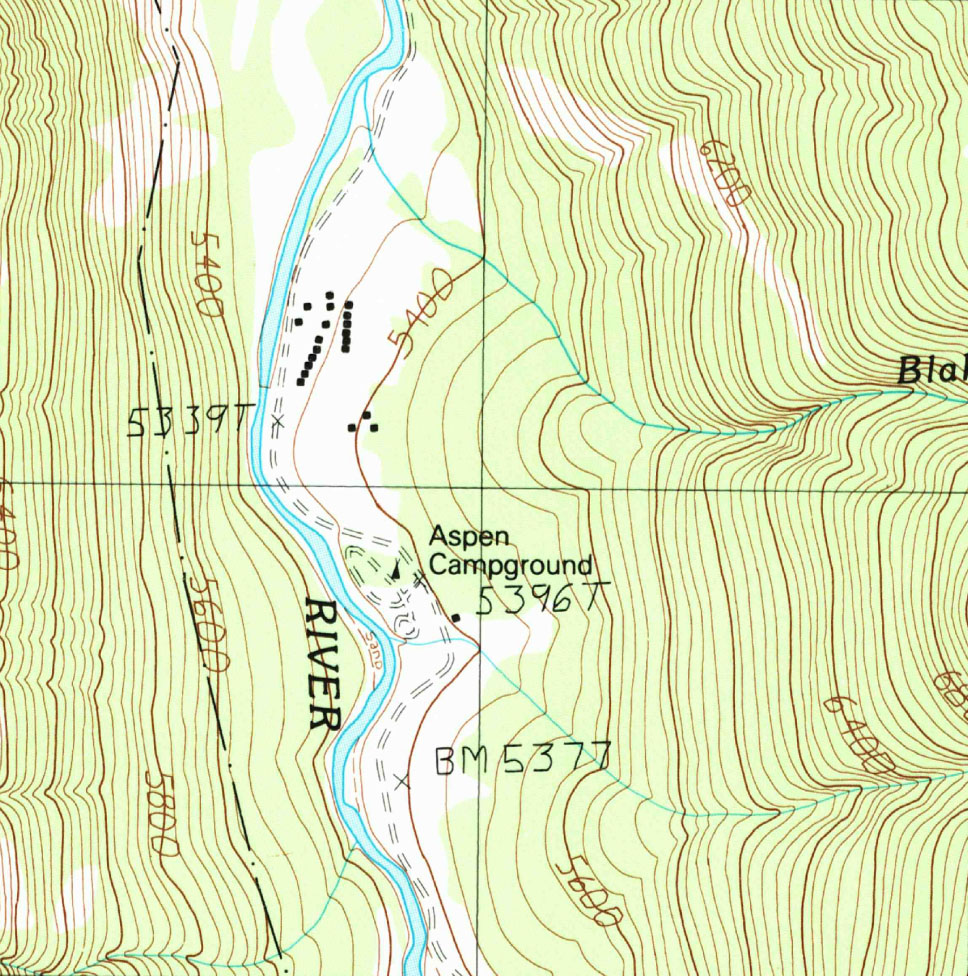
\includegraphics[scale=.65]{figures/MT_ChromeMountain_topo_small.pdf}
%}

Given a function $z=f(x,y)$, we can draw a ``topographical map'' of $f$ by drawing \textbf{level curves} (or, contour lines). A level curve at $z=c$ is a curve in the $x$-$y$ plane such that for all points $(x,y)$ on the curve, $f(x,y) = c$. 

When drawing level curves, it is important that the $c$ values are spaced equally apart as that gives the best insight to how quickly the ``elevation'' is changing. Examples will help one understand this concept.\\

\example{ex_levelcurve1}{Drawing Level Curves}{
Let $\ds f(x,y) = \sqrt{1-\frac{x^2}9-\frac{y^2}4}$. Find the level curves of $f$ for $c=0$, $0.2$, $0.4$, $0.6$, $0.8$ and $1$.}
{Consider first $c=0$. The level curve for $c=0$ is the set of all points $(x,y)$ such that $0=\sqrt{1-\frac{x^2}9-\frac{y^2}4}$. Squaring both sides  gives us
$$\frac{x^2}9+\frac{y^2}4=1,$$ an ellipse centered at $(0,0)$ with horizontal major axis of length 6 and minor axis of length 4. Thus for any point $(x,y)$ on this curve, $f(x,y) = 0$.

Now consider the level curve for $c=0.2$
\begin{align*}
0.2 &= \sqrt{1-\frac{x^2}9-\frac{y^2}4}\\
0.04 &= 1-\frac{x^2}9-\frac{y^2}4\\
\frac{x^2}9+\frac{y^2}4 &=0.96\\
\frac{x^2}{8.64}+\frac{y^2}{3.84} &=1.
\end{align*}
This is also an ellipse, where $a = \sqrt{8.64}\approx 2.94$ and $b=\sqrt{3.84}\approx 1.96$.

In general, for $z=c$, the level curve is:
\begin{align*}
c &= \sqrt{1-\frac{x^2}9-\frac{y^2}4}\\
c^2 &= 1-\frac{x^2}9-\frac{y^2}4\\
\frac{x^2}9+\frac{y^2}4 &=1-c^2\\
\frac{x^2}{9(1-c^2)}+\frac{y^2}{4(1-c^2)} &=1,
\end{align*}
ellipses that are decreasing in size as $c$ increases. A special case is when $c=1$; there the ellipse is just the point $(0,0)$. 

The level curves are shown in Figure \ref{fig:levelcurves1}(a). Note how the level curves for $c=0$ and $c=0.2$ are very, very close together: this indicates that $f$ is growing rapidly along those curves.

\mtable{.67}{Graphing the level curves in Example \ref{ex_levelcurve1}.}{fig:levelcurves1}{%
\begin{tabular}{c}
\myincludegraphics{figures/figlevelcurve1b}\\
(a)\\[10pt]
\myincludegraphicsthree{width=150pt,3Dmenu,activate=onclick,deactivate=pageinvisible,
3Droll=0,
3Dortho=0.004999999888241291,
3Dc2c=0.6562340259552002 0.7273486256599426 0.20080043375492096,
3Dcoo=2.348435640335083 -6.5163373947143555 66.12745666503906,
3Droo=129.99999641808185,
3Dlights=Headlamp,add3Djscript=asylabels.js}{}{figures/figlevelcurve1}\\
%\myincludegraphics[scale=1.25,trim=3mm 0mm 3mm 0mm,clip]{figures/figlevelcurve1}\\
(b)
\end{tabular}
}

In Figure \ref{fig:levelcurves1}(b), the curves are drawn on a graph of $f$ in space. Note how the elevations are evenly spaced. Near the level curves of $c=0$ and $c=0.2$ we can see that $f$ indeed is growing quickly.
}\\

\example{ex_levelcurves2}{Analyzing Level Curves}{
Let $\ds f(x,y) = \frac{x+y}{x^2+y^2+1}$. Find the level curves for $z=c$.}
{We begin by setting $f(x,y)=c$ for an arbitrary $c$ and seeing if algebraic manipulation of the equation reveals anything significant.
\begin{align*}
\frac{x+y}{x^2+y^2+1} &= c \\
x+y &= c(x^2+y^2+1).
\intertext{We recognize this as a circle, though the center and radius are not yet clear. By completing the square, we can obtain:}
\left(x-\frac{1}{2c}\right)^2+\left(y-\frac1{2c}\right)^2&=\frac{1}{2c^2}-1,
\end{align*}
a circle centered at $\big(1/(2c),1/(2c)\big)$ with radius $\sqrt{1/(2c^2)-1}$, where $|c|<1/\sqrt{2}$. The level curves for $c=\pm 0.2,\ \pm 0.4$ and $\pm0.6$ are sketched in Figure \ref{fig:levelcurves2}(a). To help illustrate ``elevation,'' we use thicker lines for $c$ values near 0, and dashed lines indicate where $c<0$. 

There is one special level curve, when $c=0$. The level curve in this situation is $x+y=0$, the line $y=-x$.

In Figure \ref{fig:levelcurves2}(b) we see a graph of the surface. Note how the $y$-axis is pointing away from the viewer to more closely resemble the orientation of the level curves in (a). 

\mtable{.7}{Graphing the level curves in Example \ref{ex_levelcurves2}.}{fig:levelcurves2}{%
\begin{tabular}{c}
\myincludegraphics{figures/figlevelcurve2b}\\
(a)\\[10pt]
%\myincludegraphics[scale=1.2,trim=0mm 5mm 0mm 0mm,clip]{figures/figlevelcurve2}\\
{\myincludegraphicsthree{width=150pt,3Dmenu,activate=onclick,deactivate=pageinvisible,
3Droll=0.25732633644359904,
3Dortho=0.004999999888241291,
3Dc2c=0.5196654200553894 -0.7088789939880371 0.4769051671028137,
3Dcoo=-0.7249413728713989 1.7016432285308838 3.277412176132202,
3Droo=130.00000541214214,
3Dlights=Headlamp,add3Djscript=asylabels.js}{}{figures/figlevelcurve2}}\\
(b)
\end{tabular}
}



%\mfigurethree[width=150pt,3Dmenu,activate=onclick,deactivate=pageinvisible,
%3Droll=0,
%3Dc2c=1 -1.5 1,
%3Dcoo=0 0 0,
%3Droo=130,
%3Dortho=.005,
%3Dlights=Headlamp,add3Djscript=asylabels.js]{.4}{Visualizing the solid shown from Example \ref{ex_doublepol4}.}{fig:doublepol4}{figures/figlevelcurve2_3D} 

Seeing the level curves helps us understand the graph. For instance, the graph does not make it clear that one can ``walk'' along the line $y=-x$ without elevation change, though the level curve does.
}\\

\noindent\textbf{\large Functions of Three Variables}\\

We extend our study of multivariable functions to functions of three variables. (One can make a function of as many variables as one likes; we limit our study to three variables.)

\definition{def:multi3}{Function of Three Variables}
{Let $D$ be a subset of $\mathbb{R}^3$. A \textbf{function $f$ of three variables} is a rule that assigns each triple $(x,y,z)$ in $D$ a value $w=f(x,y,z)$ in $\mathbb{R}$. $D$ is the \textbf{domain} of $f$; the set of all outputs of $f$ is the \textbf{range}.
\index{multivariable function}\index{function!of three variables}\index{multivariable function!domain}\index{multivariable function!range}
}

Note how this definition closely resembles that of Definition \ref{def:multi2}.\\

\example{ex_multi3}{Understanding a function of three variables}{
Let $\ds f(x,y,z) =  \frac{x^2+z+3\sin y}{x+2y-z}.$ Evaluate $f$ at the point $(3,0,2)$ and find the domain and range of $f$.}
{$\ds f(3,0,2) = \frac{3^2+2+3\sin 0}{3+2(0)-2} = 11.$

As the domain of $f$ is not specified, we take it to be the set of all triples $(x,y,z)$ for which $f(x,y,z)$ is defined. As we cannot divide by $0$, we find the domain $D$ is 
$$D = \{(x,y,z)\ |\ x+2y-z\neq 0\}.$$
We recognize that the set of all points in $\mathbb{R}^3$ that \textit{are not} in $D$ form a plane in space that passes through the origin (with normal vector $\la 1,2,-1\ra$). 

We determine the range $R$ is $\mathbb{R}$; that is, all real numbers are possible outputs of $f$. There is no set way of establishing this. Rather, to get numbers near 0 we can let $y=0$ and choose $z \approx -x^2$. To get numbers of arbitrarily large magnitude, we can let $z\approx x+2y$. 
}\\

\clearpage
\noindent\textbf{\large Level Surfaces}\\

It is very difficult to produce a meaningful graph of a function of three variables. A function of \textit{one} variable is a \textit{curve} drawn in \textit{2} dimensions; a function of \textit{two} variables is a \textit{surface} drawn in \textit{3} dimensions; a function of \textit{three} variables is a \textit{hypersurface} drawn in \textit{4} dimensions.\index{multivariable function!level surface}\index{level surface}

There are a few techniques one can employ to try to ``picture'' a graph of three variables. One is an analogue of level curves: \textbf{level surfaces}. Given $w=f(x,y,z)$, the level surface at $w=c$ is the surface in space formed by all points $(x,y,z)$ where $f(x,y,z)=c$. \\

\example{ex_multi4}{Finding level surfaces}{
If a point source $S$ is radiating energy, the intensity $I$ at a given point $P$ in space is inversely proportional to the square of the distance between $S$ and $P$. That is, when $S=(0,0,0)$,  $\ds I(x,y,z) = \frac{k}{x^2+y^2+z^2}$ for some constant $k$.

Let $k=1$; find the level surfaces of $I$.}
{We can (mostly) answer this question using ``common sense.'' If energy (say, in the form of light) is emanating from the origin, its intensity will be the same at all points equidistant from the origin. That is, at any point on the surface of a sphere centered at the origin, the intensity should be the same. Therefore, the level surfaces are spheres.

We now find this mathematically. The level surface at $I=c$ is defined by 
\begin{align*}
c &= \frac{1}{x^2+y^2+z^2}.
\intertext{A small amount of algebra reveals}
x^2+y^2+z^2 &= \frac1c.
\end{align*}
Given an intensity $c$, the level surface $I=c$ is a sphere of radius $1/\sqrt{c}$, centered at the origin. 

\mtable{.4}{A table of $c$ values and the corresponding radius $r$ of the spheres of constant value in Example \ref{ex_multi4}.}{fig:multi4}{
\begin{tabular}{cc}
$c$ & $r$ \\ \hline
16. & 0.25 \\
 8. & 0.35 \\
 4. & 0.5 \\
 2. & 0.71 \\
 1. & 1. \\
 0.5 & 1.41 \\
 0.25 & 2. \\
 0.125 & 2.83 \\
 0.0625 & 4. \\
\end{tabular}
}

Figure \ref{fig:multi4} gives a table of the radii of the spheres for given $c$ values. Normally one would use equally spaced $c$ values, but these values have been chosen purposefully. At a distance of 0.25 from the point source, the intensity is 16; to move to a point of half that intensity, one just moves out 0.1 to 0.35 -- not much at all. To again halve the intensity, one moves 0.15, a little more than before.

Note how each time the intensity if halved, the distance required to move away grows. We conclude that the closer one is to the source, the more rapidly the intensity changes.
}\\

\enlargethispage{2\baselineskip}
In the next section we apply the concepts of limits to functions of two or more variables.

\printexercises{exercises/12_01_exercises}